%%%%%%%%%%%%%%%%%%%%%%%%%%%%%%%%%%%%%%%%%%%%%%%%%%%%%%%%%%%%%%%%%%%%%%%%%%%%%%%%%%%%%%
%% Author:      Maximilian Stiefel
%% Date:      z  17.03.2017
%% University:  Uppsala Universitet
%% Department:  Institutionen för informationsteknologi 
%% Course:      UppSense
%% Project:     UppSens
%%%%%%%%%%%%%%%%%%%%%%%%%%%%%%%%%%%%%%%%%%%%%%%%%%%%%%%%%%%%%%%%%%%%%%%%%%%%%%%%%%%%%%

\documentclass{report}

%%%%%%%%%%%%%%%%%%%%%%%%%%%%%%%%%%%%%%%%%%%%%%%%%%%%%%%%%%%%%%%%%%%%%%%%%%%%%%%%%%%%%%
% Preamble
%%%%%%%%%%%%%%%%%%%%%%%%%%%%%%%%%%%%%%%%%%%%%%%%%%%%%%%%%%%%%%%%%%%%%%%%%%%%%%%%%%%%%%

% Encoding of the input
\usepackage[utf8]{inputenc}

% Geometry stuff
\usepackage[head=24pt,a4paper,lmargin={2.5cm},rmargin={2.5cm},tmargin={2.5cm},
bmargin={2.5cm}]{geometry}

% For graphics
\usepackage{graphicx}

% For code highlighting
\usepackage{minted}

% For shaded
\usepackage{xcolor}
\usepackage{framed}
\definecolor{shadecolor}{gray}{0.9}

% For some symbols
\usepackage{textcomp}
%\usepackage{eurosans}

% For math
\usepackage{amssymb}
\usepackage{amsmath}

\setlength{\parindent}{0em} 

% For title formatting 
\usepackage{titlesec} 

\titleformat%
{\chapter}%
[block]%
{\bfseries\Huge}%
{\thechapter\hspace{1cm}}%
{0pt}%
{\bfseries\Huge}%

% For SI units.
\usepackage{siunitx}

% Input definition macros
%%%%%%%%%%%%%%%%%%%%%%%%%%%%%%%%%%%%%%%%%%%%%%%%%%%%%%%%%%%%%%%%%%%%%%%%%%%%%%%%%%%%%%
%% Author:	Maximilian Stiefel
%% Date:	17.03.2017
%% University: 	Uppsala Universitet
%% Department: 	Institutionen för informationsteknologi 
%% Course:	UppSens
%% Project:	UppSense
%%%%%%%%%%%%%%%%%%%%%%%%%%%%%%%%%%%%%%%%%%%%%%%%%%%%%%%%%%%%%%%%%%%%%%%%%%%%%%%%%%%%%%

\newcommand{\mytitle}{Flexibel Fluorosence Intensity Measurement Platform}
\newcommand{\mytypeofwork}{Project Plan}
\newcommand{\mycourse}{UppSense} 
\newcommand{\myuniversity}{Uppsala University}
\newcommand{\mydepartement}{Information Technology}
\newcommand{\myauthora}{Elmar van Rijnswou (Elmar.Vanrijnswou.9818@student.uu.se)}
\newcommand{\myauthorb}{Maximilian Stiefel (Maximilian.Stiefel.8233@student.uu.se)}
\newcommand{\myauthorc}{}
\newcommand{\myduedate}{2017-17-10 13:00}
\newcommand{\mytutor}{Gemma Mestres (gemma.mestres@angstrom.uu.se)}
\newcommand{\mykeywords}{}
\newcommand{\myperiod}{September 2016 - September 2017}
\newcommand{\myrev}{0.2}


\usepackage{hyperref}
\hypersetup{
	plainpages=false,
	unicode=false,
	pdftoolbar=true,
	pdfmenubar=true,
	pdffitwindow=false,
	pdfstartview={FitH},
	pdftitle={\mytitle},
	pdfauthor={\myauthora ,\space\myauthorb ,\space\myauthorc},
	pdfsubject={\mytypeofwork\space\myduedate},
	pdfcreator={\myauthora ,\space\myauthorb ,\space\myauthorc},
	pdfproducer={\myauthora ,\space\myauthorb ,\space\myauthorc},
	pdfkeywords={\mykeywords},
	pdfnewwindow=true,
	pdfborder={0 0 0},
	colorlinks=false,
	linkcolor=black,
	citecolor=black,
	filecolor=black,
	urlcolor=cyan
}	

\newcommand{\newpar}{\vspace{1em}\\}
\newcommand{\myemph}[1]{\textsl{#1}}


% For PDFs
\usepackage{pdfpages}

% Header and footer
\usepackage{fancyhdr}
\lhead{\ifnum\value{chapter}>0 \includegraphics[width=1cm]{./fig/uppsla_university} \fi}
\chead{}
\rhead{\ifnum\value{chapter}>0 {\rightmark}\\\textcolor{gray}{\leftmark} \fi}
\lfoot{}
\cfoot{\ifnum\value{chapter}>0 \thepage \fi}
\rfoot{{\textcolor{red}{DRAFT}}}
\setlength{\headheight}{1cm}

\usepackage[autostyle]{csquotes}
\usepackage[style=ieee,backend=bibtex]{biblatex}
\addbibresource{literature.bib}

\begin{document}

%%%%%%%%%%%%%%%%%%%%%%%%%%%%%%%%%%%%%%%%%%%%%%%%%%%%%%%%%%%%%%%%%%%%%%%%%%%%%%%%%%%%%%
% Titlepage
%%%%%%%%%%%%%%%%%%%%%%%%%%%%%%%%%%%%%%%%%%%%%%%%%%%%%%%%%%%%%%%%%%%%%%%%%%%%%%%%%%%%%%
\input{titlepage.tex}

\newcounter{roman}
\pagenumbering{Roman}

\pagestyle{fancy}

%%%%%%%%%%%%%%%%%%%%%%%%%%%%%%%%%%%%%%%%%%%%%%%%%%%%%%%%%%%%%%%%%%%%%%%%%%%%%%%%%%%%%%
% TOC etc.
%%%%%%%%%%%%%%%%%%%%%%%%%%%%%%%%%%%%%%%%%%%%%%%%%%%%%%%%%%%%%%%%%%%%%%%%%%%%%%%%%%%%%%
\tableofcontents
\listoffigures
\newpage
\listoftables

\newpage
\setcounter{roman}{\value{page}}
\pagenumbering{arabic}
\setcounter{page}{1}

%%%%%%%%%%%%%%%%%%%%%%%%%%%%%%%%%%%%%%%%%%%%%%%%%%%%%%%%%%%%%%%%%%%%%%%%%%%%%%%%%%%%%%
% Device Description
%%%%%%%%%%%%%%%%%%%%%%%%%%%%%%%%%%%%%%%%%%%%%%%%%%%%%%%%%%%%%%%%%%%%%%%%%%%%%%%%%%%%%%
\chapter{Device Description}
\section{System Architecture}
\begin{figure}[H]
	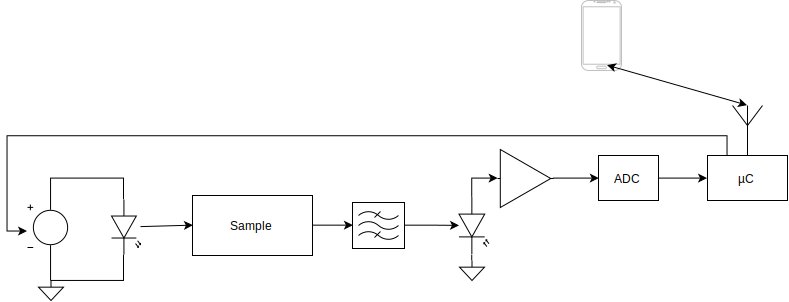
\includegraphics[width=\textwidth]{./fig/fluoresence.png}
	\caption{Rough sketch of the system architecture.}
	\label{fig:block}
\end{figure}
In figure \ref{fig:block} one can see a rough sketch of the system architecture, which is planned. The signal flow is from the left to the right. First the assay has to be excited, which is done by a voltage source connected to a light emitting diode (LED). This can also be another voltage controlled source of light. Hence this has TBD. The light source however is controlled by software (Microcontroller, µC), which is done by a simple e.g. transistor circuit. Using this approach has the advantage, that one can mix up the received signal to a higher band by switching the light source on and off with a sine wave of e.g. 1 kHz. By doing so one can suppress noise. In this case a simple mixer implemented in software can be used for instance to mix down the signal again and to process it.  
\newpar
The emitted light has to be filtered. As the wavelengths in this case are in the nm region, a optical filter is needed. Behind the filter a photo diode is located, which converts the light signal to an electrical signal. This signal probably has to be processed in a analog way (e.g. amplification and filtering) before it is transfered in the digital world (analog-digital converter, ADC). In the digital world one has a lot of possibilities. The signal will anyways be transfered to a phone via bluetooth. Moreover the phone provides huge computing capacities, which is one reason why the data should be transmitted.  

\section{Realization}
The idea is to have a printed circuit board (PCB). On this board the light source as well as the sink shall be placed on the bottom side. Ont he top side one can mount the µC and a bluetooth infrastructure. So far, a bluetooth standard shall be used to enable communication to the phone. Multiple PCBs shall be ordered, which either are having different light sources and sinks or which enable the attachement (soldering) of different light sources ands sinks. A rechargeable battery (e.g. phone battery) shall be the power source. 
\newpar
The optical filter can be mounted with epoxy resin on the PCB. Spacing bolts can be used to attach the PCB on a plate, where one can find a mechanism to easily fix the blood probe chip with that sample. Futhermore a black box which one can put over the so far depicted structure, has to be designed. This black box supresses light (noise) from the environment. Mechanical sketches have to be provided in a later revision of this document.     

\section{Frabrication}
The PCBs can be fabricated in China. This is an example of a manufacturer: \url{https://www.elecrow.com/10pcs-2-layer-pcb.html}. The lead time until one can actually work with designed PCBs is roughly three weeks including the assembling and soldering, which has to be done by the egineering subgroup.  

%%%%%%%%%%%%%%%%%%%%%%%%%%%%%%%%%%%%%%%%%%%%%%%%%%%%%%%%%%%%%%%%%%%%%%%%%%%%%%%%%%%%%%
% Budget
%%%%%%%%%%%%%%%%%%%%%%%%%%%%%%%%%%%%%%%%%%%%%%%%%%%%%%%%%%%%%%%%%%%%%%%%%%%%%%%%%%%%%%
\chapter{Budget}
\section{Prototype}
\begin{table}[H]
\centering
\begin{tabular}{lll}
\textbf{Item} & \textbf{Costs} & \textbf{Description}                                                           \\\hline
PCBs          & 50 \$          & 5 cm x 5 cm, cheapest option, which still has an acceptable quality            \\
Components    & 100 \$         & one needs to order components for the PCBs (diodes, ICs, µCs, resistors, etc.) \\
Soldering     & 0 \$           & can done by the engineering subgroup                                           \\
3D printing   & 0 \$           & for the mechanical stuff, can probably be done by Uwe                          \\
Assembling    & 0 \$           & can be done by the engineering subgroup                                       	\\\hline
\ensuremath{\sum}& 150 \$
\end{tabular}
\caption{Rough budget estimation for one prototype.}
\label{tab:prototype_budget}
\end{table}
In table \ref{tab:prototype_budget} one can see the rough costs estimation to build one prototype. This one prototype, however, subsumes multiple PCBs, which can be used for multiple assays, which have the common denominator of using a fluoresence technique. The component price also includes a lens and light source. The electrical components will roughly be 60 euros per product.
\section{Estimation Of Product Price}
The estimation of the product price depends on the techniques being used. For now there will be looked at a laser as a light source, which costs around 10 dollars. For the logic part a bluetooth service on chip(SoC) will be used. This saves cost as both the bluetooth controller and the microcontroller will be integrated in one package. The NRF52832 seems like a good pick, as knowledge about the SoC is already among the team which will increase productivity. The SoC, including passives, will cost around 15 dollar. To power everything, multiple Dc/Dc converters will be used, which will roughly come down to a price of 15 dollar. The analogue part requires a accurate high sensitive photodiode, and an amplification circuit. Which will be in the range of 15-25 dollar depending on the requirements of the photodiode. 
%%%%%%%%%%%%%%%%%%%%%%%%%%%%%%%%%%%%%%%%%%%%%%%%%%%%%%%%%%%%%%%%%%%%%%%%%%%%%%%%%%%%%%
% Gantt
%%%%%%%%%%%%%%%%%%%%%%%%%%%%%%%%%%%%%%%%%%%%%%%%%%%%%%%%%%%%%%%%%%%%%%%%%%%%%%%%%%%%%%
\chapter{Research}
In order to facilitate all the functionality, some research will be done to acquire the required knowledge. This research will be targeted towards three fields: Analogue processing, Digital communications, reception of real world signals.
\section{Reception}
The real world signal will have to be translated into an electrical signal. This can be either analogue or digital, depending on the sensors used. Different photodiodes are available on the market. Some of which contain a filter. Investigation has to be done to get a better understanding of the filters, and what drawbacks there are when buying a photodiode with filter vs buying a photodiode without. Also some photodiodes contain an internal ic that either does amplification and/or analogue-digital conversion. Once the real world signal has been converted to a electrical signal, it will have to be amplified. The signal will possibly have to be translated to a digital value, depending on the requirements and capabilities of the microcontroller.
\section{Processing}
The modulating of the light source will have to be investigated. If this is a option that indeed will increase the signal to noise level, then the effect will have to be demodulated on the microcontroller. Once this is done other filter designs might have to be implemented depending on the quality and fluctuation of the incoming signal.
\section{Communications}
Once all this information is available, a way to show it to the user has to be developed. This will be done trough bluetooth, as discussed in earlier chapters. More information has to be gathered about the different bluetooth attributes and whether available Generic Attributes (GATT) can be used or if a serial connection is required. A serial connection would require some sort of higher level protocol, which also has to be looked into. Once the information is received by the mobile phone of the designated user it will have to be processed and shown on the screen.
%%%%%%%%%%%%%%%%%%%%%%%%%%%%%%%%%%%%%%%%%%%%%%%%%%%%%%%%%%%%%%%%%%%%%%%%%%%%%%%%%%%%%%
% Gantt
%%%%%%%%%%%%%%%%%%%%%%%%%%%%%%%%%%%%%%%%%%%%%%%%%%%%%%%%%%%%%%%%%%%%%%%%%%%%%%%%%%%%%%
\chapter{Gantt}
A Gantt chart will be produced after Wednesday 29th of march, as new information will be obtained which is crucial for specifics of the project.
\printbibliography[heading=bibintoc]

\clearpage
\pagenumbering{Roman}
\setcounter{page}{\value{roman}}
\pagestyle{empty}
%%%%%%%%%%%%%%%%%%%%%%%%%%%%%%%%%%%%%%%%%%%%%%%%%%%%%%%%%%%%%%%%%%%%%%%%%%%%%%%%%%%%%%
% Appendix
%%%%%%%%%%%%%%%%%%%%%%%%%%%%%%%%%%%%%%%%%%%%%%%%%%%%%%%%%%%%%%%%%%%%%%%%%%%%%%%%%%%%%%
\appendix
% Introduce new geometry to be able to have more space for appendix
\newgeometry{lmargin={2.5cm},rmargin={2.5cm},tmargin={0cm},bmargin={1,5cm}}

\end{document}
